%\RequirePackage{fixltx2e}
%\documentclass[floatfix,aps,prd,amsmath,amssymb]{revtex4}
%\usepackage{graphicx}
%\usepackage{caption}
%\usepackage{subcaption}
%\captionsetup{compatibility=false}
%\usepackage[noabbrev,capitalise]{cleveref}
%\usepackage{hyperref}
%\begin{document}
\section{The CKM Mechanism}
\vspace{-1.0em}
\begin{center}
\tiny{\textit{John Ronayne}}
\end{center}

The weak force allows the change of flavor of say an up quark to a down quark. A deeper connection in the standard model can be made when we relate this to the electron and electron neutrino transitions \cite{CKM8}. It was originally noted by Nicola Cabibbo that the strengths of these processes were remarkably similar to within 4$\%$. This discrepancy however bore some real consequences. It was the assumption of the existance of a charm quark and 3rd generation of quarks by Kobayashi and Maskawa that noted this 4$\%$ uncertainty had some real significance and this difference didn't simply disappear with more accurate readings. The ability of the Weak force to decay between the generations explained this reduction in the strength of the decay amplitude. This has some rather interesting features. One can make use of Pythagoras' theorem to determine a unique angle between each decay path, known as the Cabibbo angle. If two generations were the full story we would envision that \cref{cabibbo} would be the principal triangle.

\begin{figure}[h]
\centering
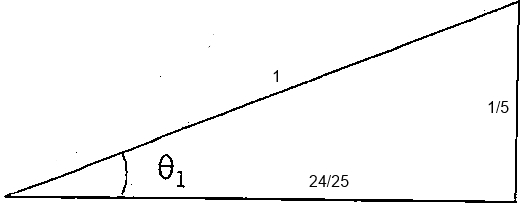
\includegraphics[angle=1, width=0.4\textwidth]{figs/ckmfig1.jpg}
\caption{Cabibbo angle $\theta_1$. Lengths represent decay amplitudes}
\label{cabibbo}
\end{figure}

Only one thousandth of the $4\%$ deviation here is accountable from the 3rd generation but for the moment lets look a bit more into the first two generations.
It shall be shown that these subtle effects arising from the 3rd generation decay amplitudes are where the theory upon CP violation was developed from. From \cref{cabibbo} it is seen that the transition within a generation $u\rightarrow d$ is calculated as $\cos\theta$ and across the generation as $\sin\theta$ which actually corresponds to $u\rightarrow s$. Naively presuming only two generations of matter existed, constructing and amplitude matrix of the corresponding transitions based on this would be appropriate, as will be demonstrated in Eqn.(\ref{mat1}). Note that, for the moment, anti-particles have amplitudes that are the same as their matter counterparts \cite{CKM1}.

\begin{equation}\label{mat1}
\left( \begin{array}{ccc} 
A_{ud} & A_{us} \\
A_{cd} & A_{cs}  \\
\end{array} \right)
 = \left( \begin{array}{ccc}
 \cos\theta_{1} & \sin\theta_{1} \\
 -\sin\theta_{1} & \cos\theta_{1} \end{array} \right)\end{equation}

From \cref{cabibbo} it is calculated that $\theta_1\sim 12^{\circ}$. Experimentally this is measured $\theta_1 = 13.1^{\circ}$ \cite{CKM9}.The impact of this was that the decay rate of many hadronic particles could be calculated, akin to lepton decays, with the additional factor of $\cos\theta_1$or $\sin\theta_1$ in the matrix element. At a quick glance of the Weak Lagrangian,
\begin{equation}\label{mat2}
L_{weak} = i\bar{\psi}\gamma^{\mu}(1-\gamma^{5})\partial^{\mu}\psi -q\sum\bar{\psi}\gamma^{\mu}\sigma_{i}(1-\gamma^{5})\psi A_{\mu i} -\frac{1}{4}F_{\mu \nu}F^{\mu \nu}
\end{equation} 
 the interaction term (the second term in Eqn.(\ref{mat2})) is a key element in the vertexes of the Feynman diagram describing the interactions in \cref{fey1}. An element of this, $\gamma$, signifies axial vector coupling with properties which contribute to CPV \cite{CKM2}.

\begin{figure}[h]
\centering
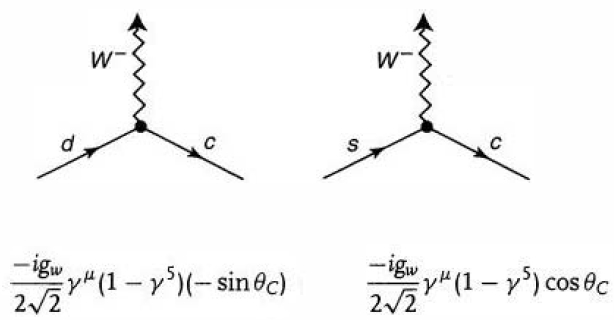
\includegraphics[width=0.5\textwidth]{figs/ckmfig2.jpg}
\caption{Decay amplitudes across generations (Note the Cabbibo angle $\theta_c$ =$\theta_1$). Left $d\rightarrow c$ and right $s\rightarrow c$.}
\label{fey1}
\end{figure}


To progress onto a mechanism for mixing 3 generations of quarks, the first steps must look further into what sets the weak interacting quarks apart from the quarks that are involved in electromagnetic and strong interactions. To begin let us look at an example of the kaon decay into two muons.

\begin{figure}[h]
\centering
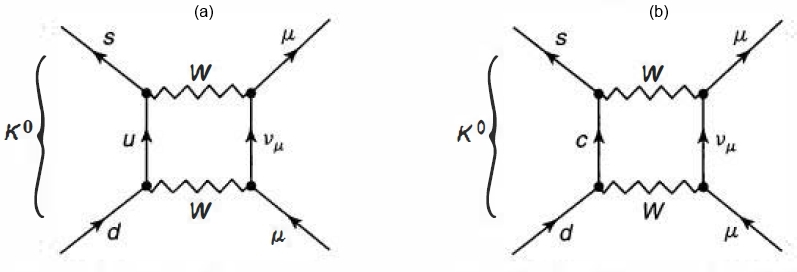
\includegraphics[width=0.5\textwidth]{figs/ckmfig3.jpg}
\caption{Kaon Interfering Feynamn diagrams illustrating GIM mechanism}
\label{fey2}
\end{figure}


So for a decay scheme as the Kaon in \cref{fey2}.a , the virtual up quark is what will be transmitted between the down and strange. This is what would be know as a second order diagram, since the direct decay to a W boson is forbidden. When the amplitudes are found the branching ratio between that and the $K^+\rightarrow\mu\nu$ is calculated to be,
\begin{equation}\label{mat3}
 \frac{K^0\rightarrow\mu\mu}{K^+\rightarrow\mu\nu}=10^{-8}.
\end{equation}
However experimentally this value is found to be too high. What could also be possible is the diagram in \cref{fey2}.b where the virtual quark is now charm. When taking into account these two process we find that in \cref{fey2}.a the amplitude is proportional to $\sin\theta_1 \cos\theta_1$ and in \cref{fey2}.b the amplitude is proportional to $-\sin\theta_1 \cos\theta_1$ on account of $A_{cd}$ in our simple matrix above \cite{CKM5}. 
In 1970, what is called the (Glashow, Iliopoulos and Maiani) GIM mechanism was responsible for a solution \cite{CKM9}. It proposed that ,through the interference with another possible decay process (or diagram) there would be a near cancellation. The remaining value came from the difference in mass between the up and charmed quark. Using the experimental Amplitudes this allowed calculations and clear predictions for the mass of the charmed quark of about $1.5GeV$. It was successfully discovered in 1974 which then ushered what was known as the November Revolution \cite{CKM2}.
 \\
\\
Cabibbo's theory of mixing together with the GIM mechanism allows for an insightful view of quarks from a different perspective. Instead of one quark that feels the strong, electromagnetic and weak force, there is a sort of mixed phase of quarks involved in weak interactions. So an incognito weak d and s are given by,

\begin{equation}\label{wd}
d' =d\cos\theta_1 +s\sin\theta_1
\end{equation}
 and
\begin{equation}\label{ws}
s'=s\cos\theta_1 -sin\theta_1.
\end{equation}
This can then formulate the matrix,
\begin{equation}\label{mix}
 \left( \begin{array}{c} d' \\  s' \end{array} \right)  = \left( \begin{array}{ccc} cos\theta_1 & sin\theta_1 \\ -sin\theta_1 & cos\theta_1 \end{array}\right) \left( \begin{array}{c} d \\  s \end{array} \right)
\end{equation}
Now the following doublets are found like in leptons using an analogous Cabibbo rotated states,

\begin{equation}\label{mix1}
\left( \begin{array}{c}
 u \\ d'
 \end{array} \right)  = 
\left( \begin{array}{c}
 u \\ d\cos\theta_1 +s\sin\theta_1
 \end{array} \right) \mbox{ and }
 \left( \begin{array}{c}
 c \\ s' \\
 \end{array} \right)  =
 \left( \begin{array}
{c} c \\
 s\cos\theta_1 -d \sin\theta_1 \\
 \end{array}
\right)
\end{equation}
Moving onto a third generation of quarks, the method of finding mixing angles from the Amplitude triangles is repeated.
\begin{figure}[h]
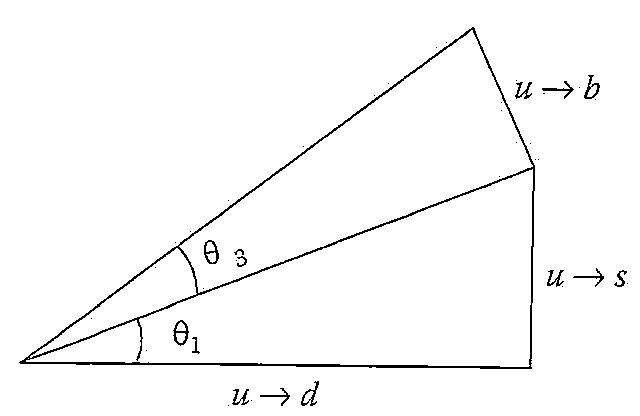
\includegraphics[width=0.3\textwidth]{figs/ckmfig4a.jpg}
\caption{Mixing triangle across 3 generations}
\label{tri3}
\end{figure}

\begin{figure}[h]
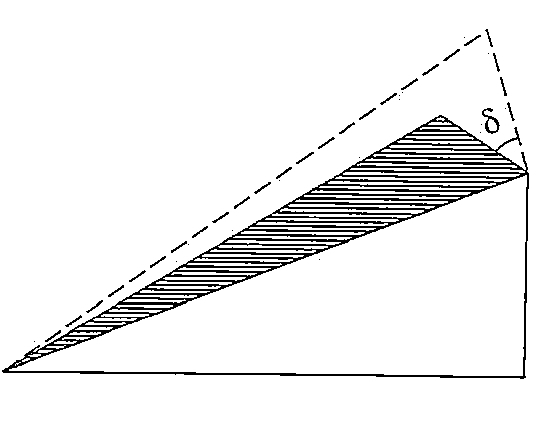
\includegraphics[angle=1.1,width=0.3\textwidth]{figs/ckmfig4b.jpg}
\caption{Complex phase in the 2nd to 3rd generation transitions}
\label{tri4}
\end{figure}

In \cref{tri3} what now is in place is an additional triangle with its base atop the hypotenuse of the 1st to 2nd generation triangle. The transition now facilitates the Amplitude of the up quark transitioning towards the bottom quark path. This gives rise to the angle $\theta_3$ a mixing angle between the 1st and 3rd generation and proceeding with this convention the mixing angle between the 2nd and 3rd is naturally $\theta_2$. The pictorial representation has another hidden feature, \cref{tri4}. The plane the triangle sits in can be thought of as the ‘matter-antimatter mirror’ with the addition freedom of the upper right-angle triangle to swing in and out of the page at an angle $\delta$. It is called the Kobayashi-Maskawa phase, where $\delta=0$ is on the plane of the triangle below. This parameter can set a difference between preferred taste of flavor (quarks and anti-quarks) which will later be shown in Section[IV] and may be the clue to the source of CP violation in nature and perhaps even the structure of the universe itself, but that remains to be seen since in Section[VI] and Section[VII] while still abiding to the conditions that are in place to allow for CP violation , $\delta\neq0$,$\pi$ or $\theta_i\neq0,\frac{\pi}{2}$  \cite{CKM4} .
With a full catalog of mixing between quarks, scaling the prior models to a 3x3 matrix is a task performed in \cite{CKM3} , it incorporates every type of quark mixing in the original formalism. 

\begin{equation}\label{ckm1}
V_{CKM} = \left( \begin{array}{ccc} V_{ud} & V_{us} & V_{ub} \\ V_{cd} & V_{cs} & V_{cb} \\ V_{td} & V_{ts} & V_{tb} \end{array}\right) = \left( \begin{array}{ccc} c_1 & s_1 c_3 & s_1 s_3 \\ -s_1 c_2 & c_1 c_2 c_3 -s_2 s_3 e^{i\delta} & c_1 c_2 s_3 + s_2 c_3 e^{i\delta} \\ -s_1 s_2 & c_1 s_2 c_3 +c_2 s_3 e^{i\delta} & c_1 s_2 s_3 - c_2 c_3 e^{i\delta} \end{array} \right). 
\end{equation}

In order to take advantage of the CKM matrix and illuminate CP violating decays,  two weak amplitudes with complex phase components must exist. An example of such would be the model 4 quark system \cite{CKM4}. Consider two up quarks i and k and two down quarks j and l. Its possible to find that the matrix element is,

\begin{equation}\label{mat4}
M=(V_{ij} V_{kl}) A_1 e^{i \delta_{1}} +(V_{il} V_{kj}) A_2 e^{i\delta_{2}}
\end{equation}

Where $A_1$ and $A_2$ are real value amplitudes and each one represents a unique initial state transitioning to the same final states .The $\delta_1$ and $\delta_2$ are the phases due to higher order processes. The difference between them may be defined as the $\Delta\delta = \delta_1 - \delta_2$ and is known as the CP-even phase. Performing the $\bar{C}\bar{P}$ operation on this matrix element a new one is obtain,

\begin{equation}\label{mat5}
\overline{M}=(V_{ij} V_{kl})^* A_1 e^{i\delta_1} +(V_{il} V_{kj})^* A_2 e^{i\delta_2}
\end{equation}

The two individual amplitudes $A_1$ and $A_2$ in each of the Matrix elements interfere with each other, so to simplify this down for a moment let us absorb the coefficients into $A_1$ and $A_2$ and solve for their decay rates \cite{CKM6}. 
Let,
\begin{equation}\label{amp1}
 \left|A\right|^2 = \left| A_1 +A_2 \right|^2 =\left|  A_1 \right|^2+ \left| A_2 \right|^2 +2\it{R} e\left| A^*_2 A_1 \right| 
\end{equation}

\begin{equation}\label{amp2}
 =\left| A_1 \right|^2 + \left| A_2 \right|^2 +2\left|A_1 A_2 \right| cos(\Delta \phi - \Delta\delta),
\end{equation}
 and
\begin{equation}\label{amp3}
\left| \overline{A}\right|^2 =\left| A_1 \right|^2+ \left| A_2 \right|^2 +2\left| A_1 A_2 \right| cos(\Delta \phi - \Delta\delta),
\end{equation}


The $\phi$ in this case is the CP-even phase. Now defining the CP asymmetry as,

\begin{equation}\label{As1}
\mathbf{A}_{CP} = \frac{\left|A\right|^2-\left|\overline{A}\right|^2}{\left|A\right|^2+\left|\overline{A}\right|^2}
\end{equation}

Apply equation \ref{As1} to \ref{mat4} and \ref{mat5} to find the Asymmetry in our four quark system we solve for the matrix elements. The result is,

\begin{equation}\label{Asm1}
 \mathbf{M}_{CP}= \frac{ 2\it{I}m (V_{ij} V_{kl} V^{*}_{kj }V^{*}_{il} )\sin(\Delta\delta) A_{1} A_{2}}{\left| V_{ij} V_{kl}\right|^2 A^{2}_{1} + \left|V_{kj}V_{il}\right|^2 A^{2}_{2} +2 \it{R} e (V_{ij} V_{kl} V^{*}_{kj} V^{*}_{il} ) \cos(\Delta\delta)A_1 A_2}
\end{equation}\

CP violation in this respect is proportional to $2\it{I}m(V_{ij}V_{kl}V^{*}_{kj}V^{*}_{il})$ which is called $\cal{J}$, the Jacobian. The Jacobian is just the gradient of the scalar valued CKM matrix it also is subject to the same CP violating conditions as what $\delta$ boasted.

So now it may same possible to be stuck with the eternal burden of having a theory with an unknown number of free parameters to test with. To fix this we would like our CKM matrix to be unitary i.e. that itself by it's complex conjugate produces the Identity matrix. A quick glance and a brief frown reveals that the matrix thus far bare no hope unless our off-diagonal elements are relatively small. Hence since CP violation turns out to be very small experimentally and these off diagonal elements are in turn correlated to CPV it has been constructed, in close approximation, a unitary matrix as such. Adopting the Wolfenstein parametrization \cite{CKM10} where we expand on a small parameter $\lambda = 0.22$ to a power series,

\begin{equation}\label{VW1}
V_{W} =\left| \begin{array}{ccc} 1-\frac{\lambda^2}{2} & \lambda & A\lambda^3(\rho-i\nu) \\ -\lambda & 1-\frac{\lambda^2}{2} & A\lambda^2 \\ A\lambda^3(1-\rho-i\nu) &  -A\lambda^2 & 1 \end{array}\right| + {\cal{O}}(\lambda^{4})
\end{equation}
Looking back at the original CKM matrix in \ref{ckm1},
\[\lambda =s_{1}\mbox{  ,    } A=\frac{s_{2}}{s^{2}_{1}}\mbox{  ,    } \rho =\frac{s_{3}}{s_{1}s_{2}}\cos\delta \mbox{ and } \nu = \frac{s_3}{s_1}{s_2}\sin\delta.\]
Comparing this to experimentally measured values CKM matrix elements we have pretty close agreement.
\begin{equation}\label{VEXP1}
V_{exp} = \left( \begin{array}{ccc} 0.9739-0.975 & 0.221-0.227 & 0.0029-0.0045 \\ 0.221-0.227 & 0.9730-0.9744 & 0.039-0.044 \\ 0.0048-0.01 &  0.037-0.043 & 0.9990-0.9992 \end{array}\right) + {\cal{O}}(\lambda^{4})
\end{equation}
\\
As you can see there is a dependence on experimental data but to what extent is it needed. An $n\times n$ complex matrix will have $n^2$ real and complex parameters while unitarity meaning we have $n^2$ constrains. Since we have 6 quarks $(2n)$ which can all have independent phases we have $2n$ fewer parameters. Fixing one phase we then have $n^2 - (2n - 1)$. In the real unitary matrix we have n dimensions and $\frac{n(n-1)}{2}$ free parameters. Thus the total imaginary parameters in the CKM matrix is,
\begin{equation}\label{par1}
n^2 - (2n - 1)-\frac{n(n-1)}{2} = \frac{(n-1)(n-2)}{2}
\end{equation}
 which for n=3 is 1. Hence we have 4 unknown parameters in total, which is why the values of the CKM matrix depend on experimental constraints \cite{CKM7}
\\

As found in \cite{CKM5}, 9 constraints are needed, 6 of which are the sum of complex terms which are zero by orthogonality.  Here are three of these unitary relation equations, 
\begin{equation}\label{par2}
V_{ud}V^{*}_{us}+V_{cd}V^{*}_{cs}+V_{td}V^{*}_{ts}=0,
\end{equation}
\begin{equation}\label{par3}
V_{us}V^{*}_{ub}+V_{cs}V^{*}_{cb}+V_{ts}V^{*}_{tb}=0,
\end{equation}
\begin{equation}\label{par4}
V_{ud}V^{*}_{ub}+V_{cd}V^{*}_{cb}+V_{td}V^{*}_{tb}=0,
\end{equation}

A way to visualize these is as the Unitary triangles in the complex plane and have a surface area of $\frac{\left|\cal{J}\right|}{2}$ \cite{CKM11}. The area is then non-zero for CP violating weak interactions.

\begin{figure}[h]
\centering
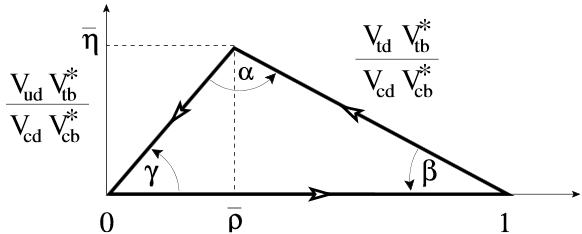
\includegraphics[width=0.5\textwidth]{figs/ckmfig5.jpg}
\caption{Unitary Triangle with angles $\alpha, \beta \mbox{ and } \gamma$}
\label{tri4}
\end{figure}
Now to look a bit closer at the unitary Eqn.(\ref{par4}) to construct the appropriate triangle. In \cref{tri4} a triangle on the basis (x,y) with corners at (0,0), (1,0) and ($\overline{\rho},\overline{\nu}$) is formed, where the reparameterizations are,

\begin{equation}\label{pv1}
\overline{\rho}=\rho\left(1-\frac{\lambda^2}{2}\right) \mbox{ and } \overline{\nu}=\nu\left(1-\frac{\lambda^2}{2}\right)
\end{equation}
The three angles in this diagram $\alpha , \beta \mbox{ and } \gamma$ are defined as,

\begin{equation}\label{ang1}
 \alpha\equiv arg\left(-\frac{V_{tb}V^{*}_{tb}}{V_{ud}V^{*}_{ub}}\right) =\frac{1}{2}\sin^{-1}\left(\frac{2\overline{\nu}(\overline{\nu}^2+\overline{\rho}^2-\overline{\rho})}{(\overline{\rho}^2+\overline{\nu}^2)((1-\overline{\nu})^2+\overline{\nu}^2)}\right) .
\end{equation}

\begin{equation}\label{ang2}
\beta\equiv argl\left(-\frac{V_{cd}V^{*}_{cb}}{V_{td}V^{*}_{tb}}\right) = \frac{1}{2}\sin^{-1}\left(\frac{2\overline{\nu}(1-\overline{\rho})}{(1-\overline{\rho})^2+\overline{\rho}^2}\right).
\end{equation}

\begin{equation}\label{ang3}
\gamma\equiv arg\left(-\frac{V_{ud}V^{*}_{ub}}{V_{cd}V^{*}_{cb}}\right) = \frac{1}{2}\sin^{-1}\left(\frac{2\overline{\rho}\overline{\nu}}{\overline{\rho}^2+\overline{\nu}^2}\right).
\end{equation}

and $\alpha + \beta + \gamma = 180^{\circ}$. Direct measurement of these angles is performed by observations of CP violations in B,D and Kaon meson decays which shall be covered in the following sections \cite{CKM7}.
